%1BRSa
\begin{figure}[h]
    \centering
    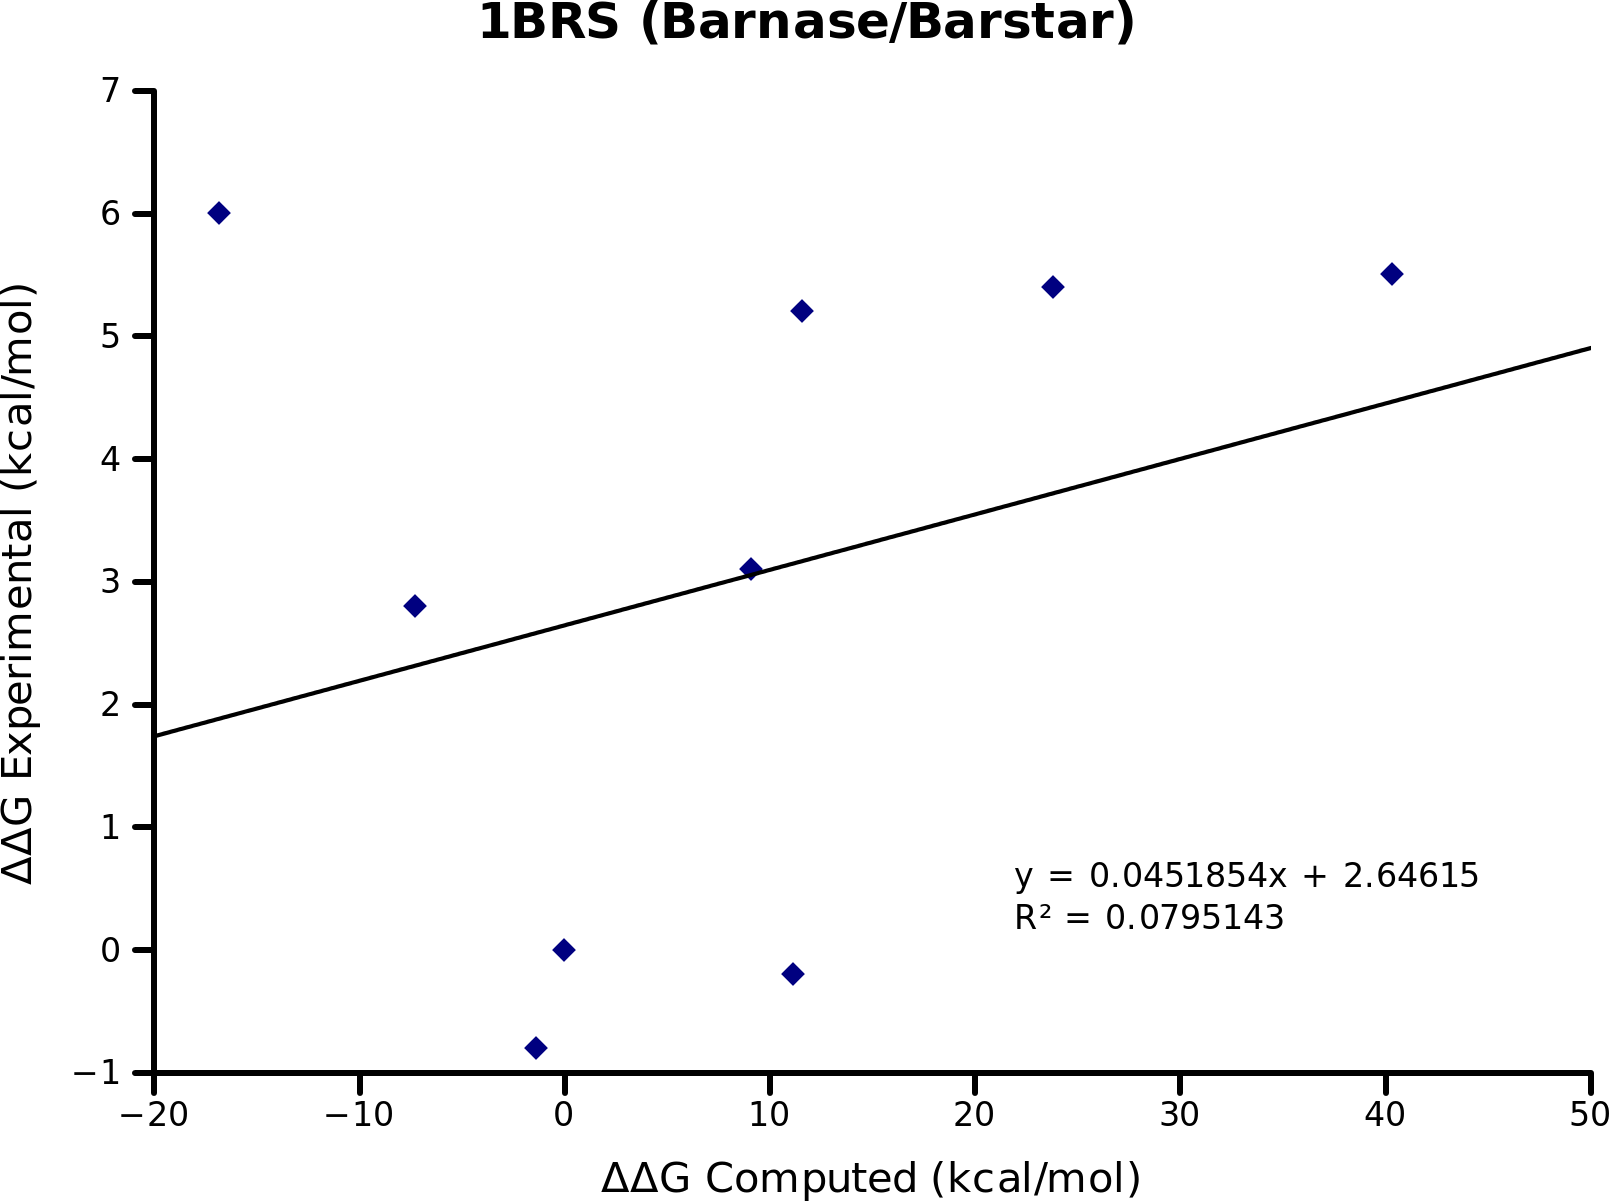
\includegraphics[width=0.65\textwidth]{figures/1brs_barnase_barstar.png}
    \caption{Computed versus experimental \ddg\ binding for 8 alanine mutations in the Barstar-Barnase binding pair.
    Crystal structure used for computations was 1BRS.
    Specific amino acids mutated were residues 27, 54, 58, 59, 60, 73, 87, and 102, all of chain A.
    Experimental binding affinity taken from \protect\cite{thorn2001asedb}.}
    \label{figure:computational_mutation_scanning/1BRSa_ddg}
\end{figure}

\begin{table}[H]
\centering
\label{table:1brs_a_results}
\begin{tabular}{|c|c|c|}
\hline
Residue & \ddg\ calculated & \ddg\ experimental \\
\hline
native & 0 & 0 \\
27 & 23.82 & 5.4 \\
54 & -1.37 & -0.8 \\
58 & 9.09 & 3.1 \\
59 & 11.58 & 5.2 \\
60 & 11.15 & -0.2 \\
73 & -7.28 & 2.8 \\
87 & 40.32 & 5.5 \\
102 & -16.83 & 6 \\
\hline
\end{tabular}
\caption{}
\end{table}

\begin{table}[h]
\centering
\begin{tabular}{|c|c|c|}
\hline
Residue & Amino Acid & RMSD \\
\hline
A:27 & LYS & 1.213 \\
A:54 & ASP & 0.920 \\
A:58 & ASN & 0.121 \\
A:59 & ARG & 0.421 \\
A:60 & GLU & 0.138 \\
A:73 & GLU & 0.994 \\
A:87 & ARG & 0.297 \\
A:102 & HIS & 0.276 \\
\hline
\end{tabular}
\caption{RMSD of mutated side chains in barnase, in a barnase-barstar complex (chain A of PDBid 1BRS), during the mutation scanning experiments.}
\label{table:1BRSa_rmsd}
\end{table}


\begin{figure}[h]
    \centering
    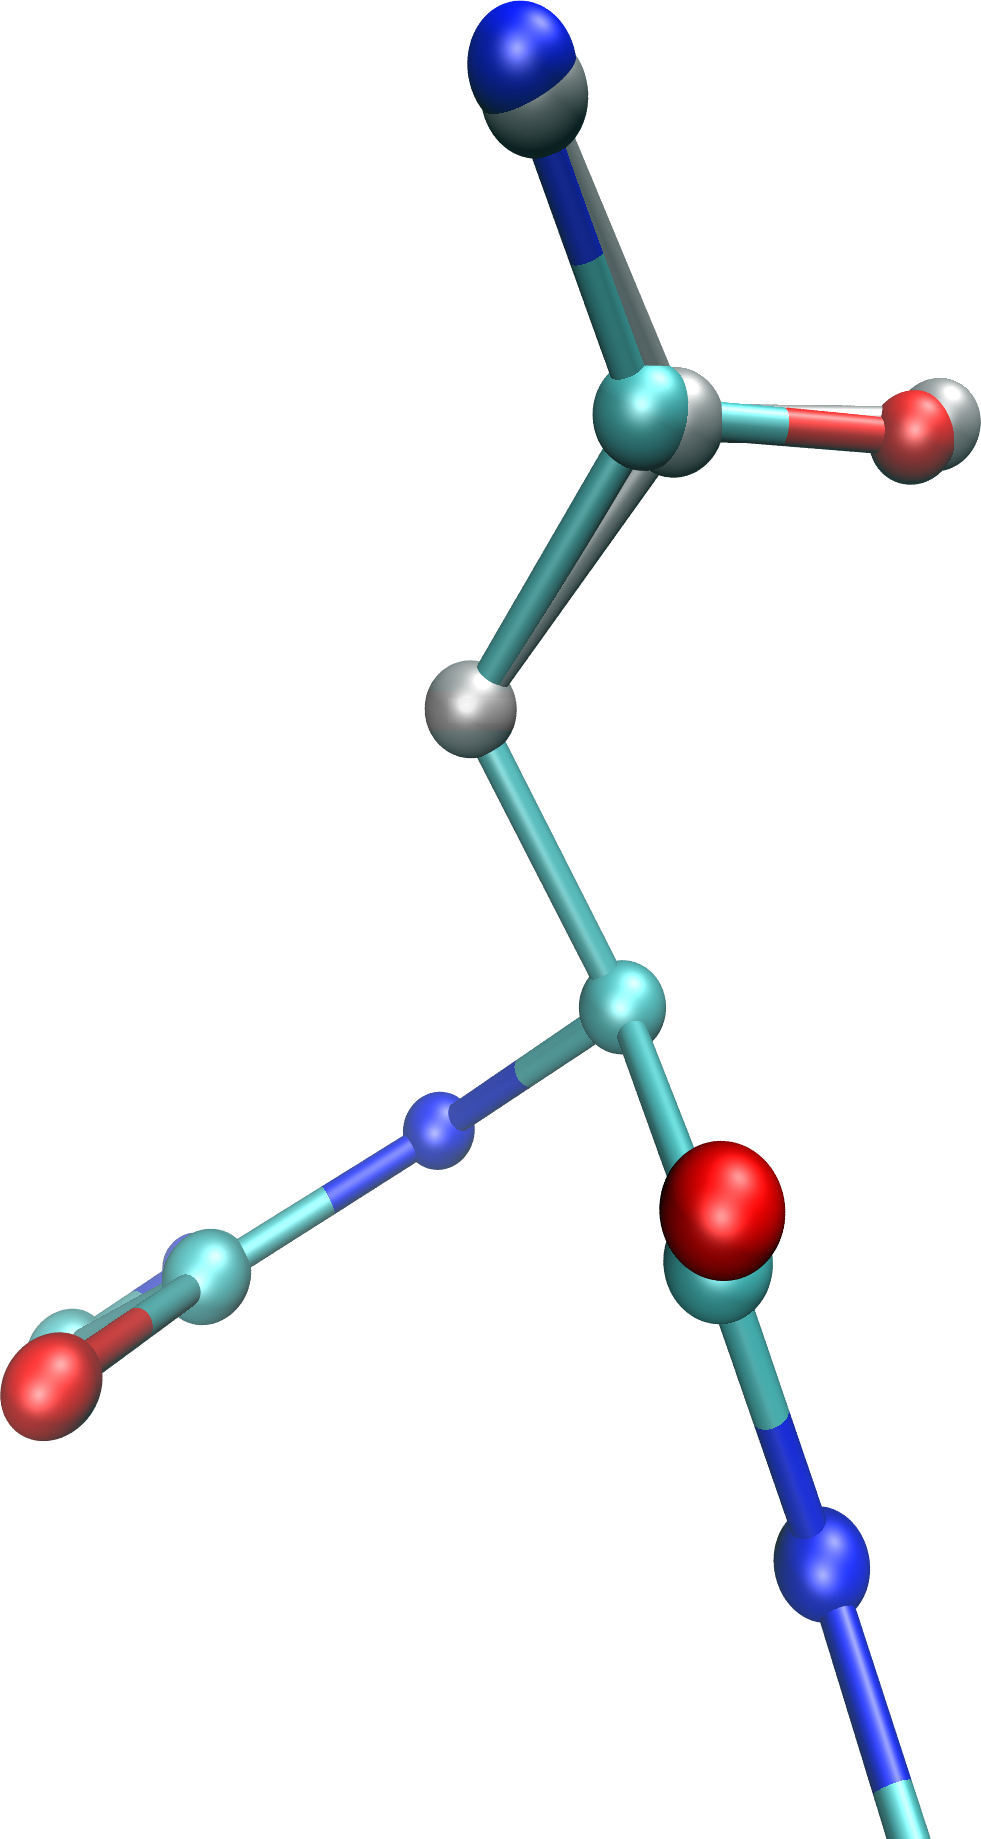
\includegraphics[width=0.65\textwidth,height=0.3\textheight,keepaspectratio]{figures/mutation_side_chain_images/1brs_chain_a_resid_58.png}
    \caption{Crystal, colored by atom, and predicted, magenta, side chain conformations for barnase, asparagine 58 of 1BRS.
    The predicted and crystal conformations are almost identical, differing by only 0.121 angstroms, or less than the resolution of the crystal structure.}
    \label{figure:computational_mutation_scanning/1brs_a_58}
\end{figure}

\begin{figure}[h]
    \centering
    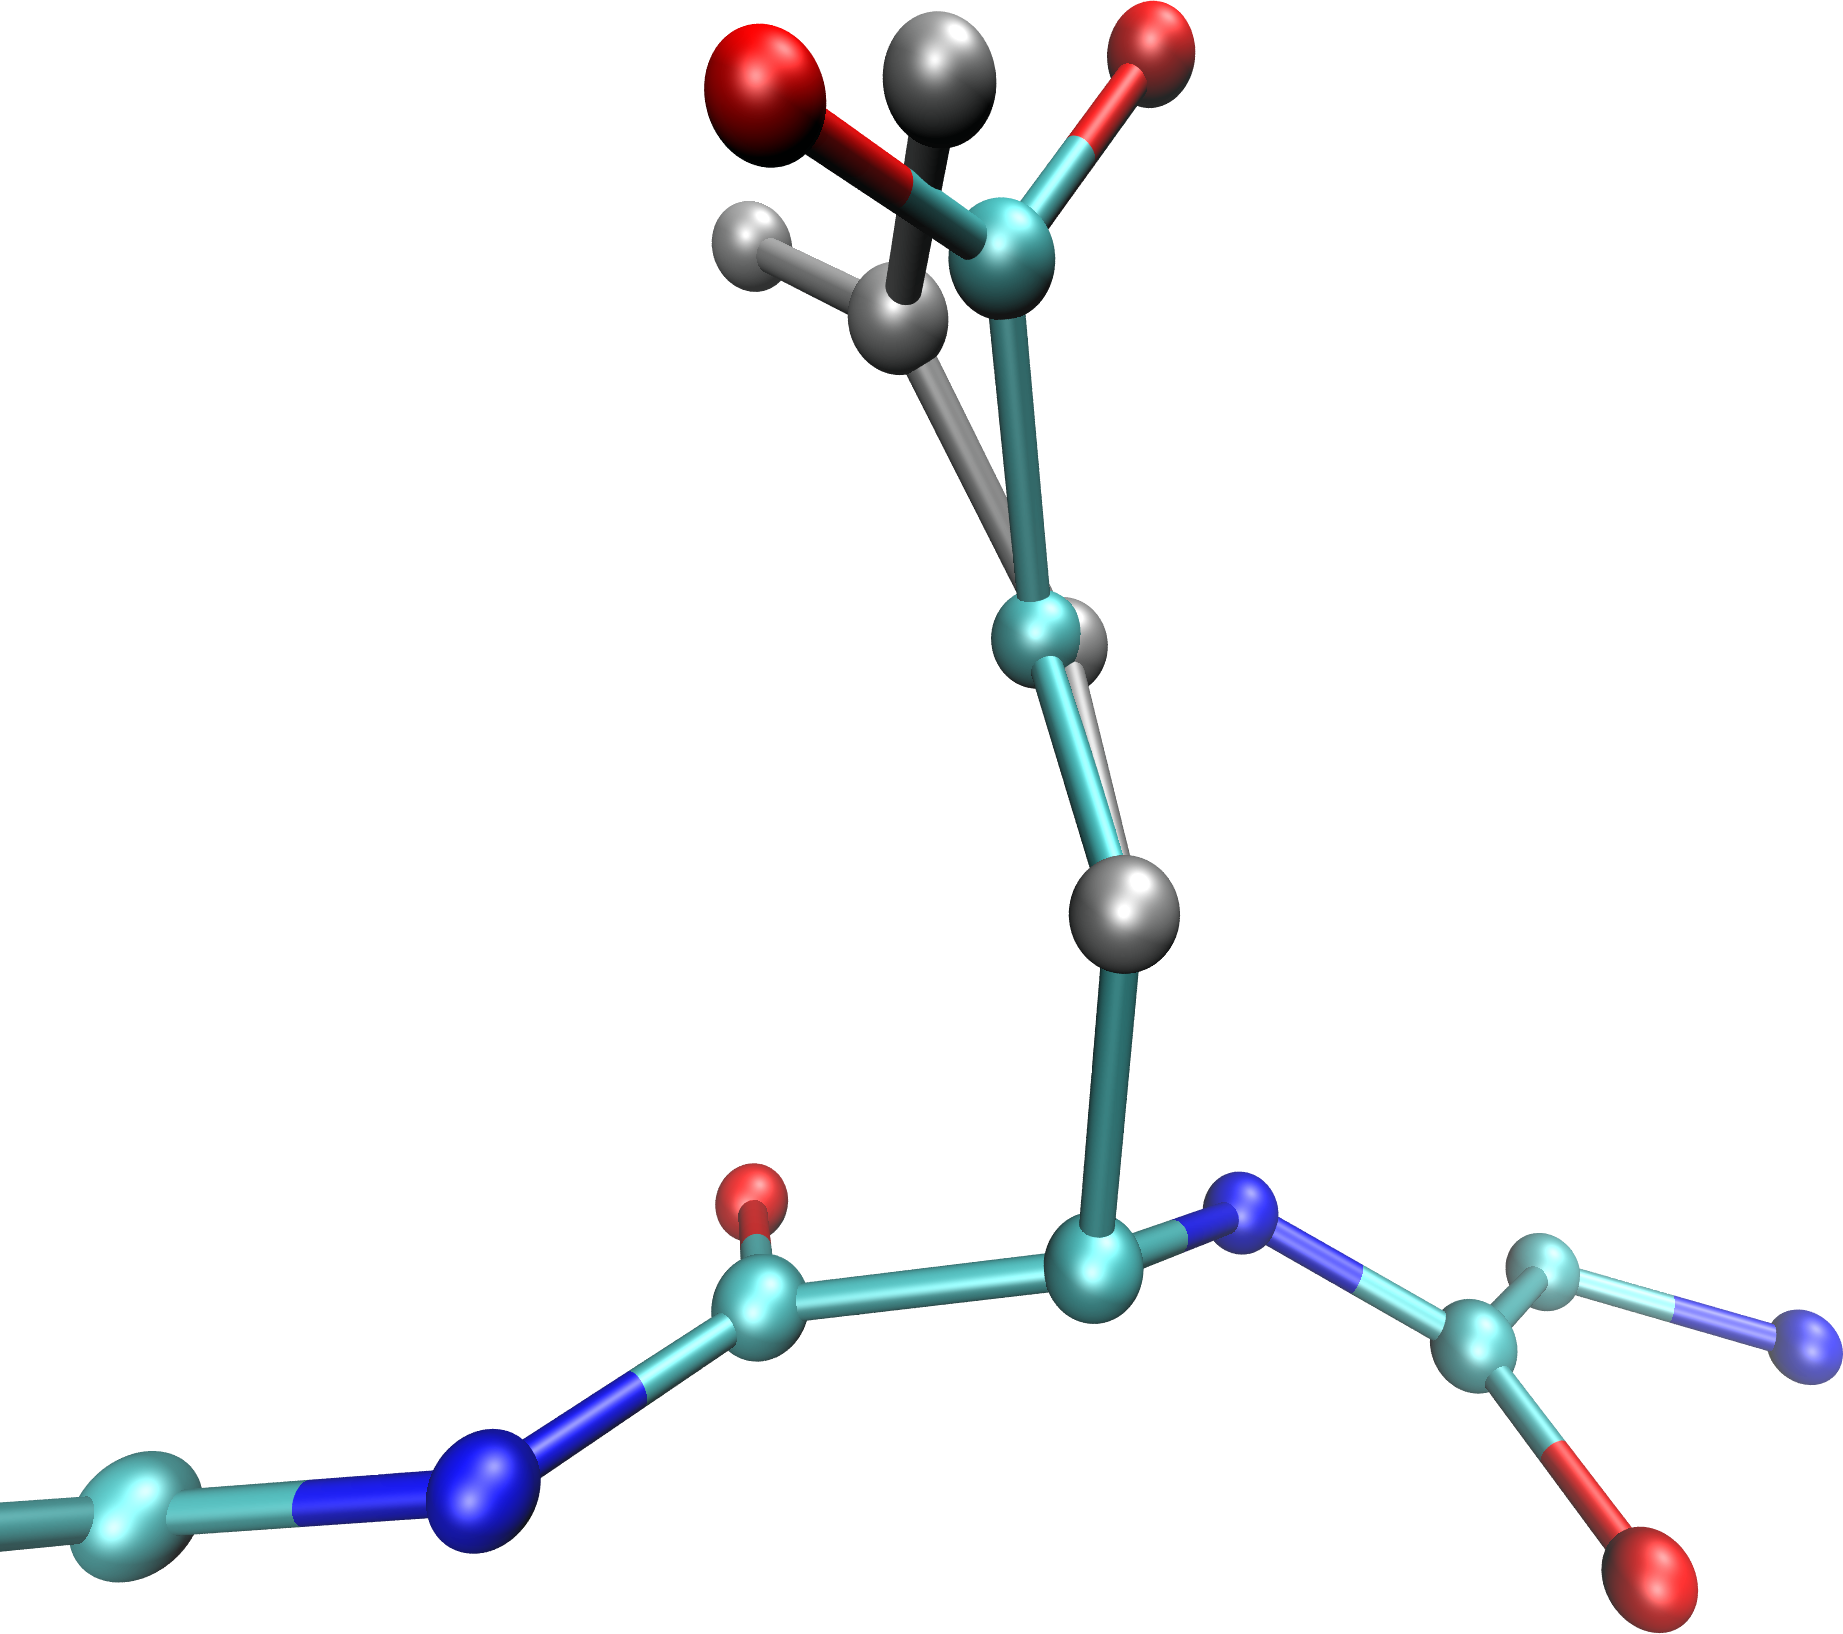
\includegraphics[width=0.65\textwidth,height=0.3\textheight,keepaspectratio]{figures/mutation_side_chain_images/1brs_chain_a_73.png}
    \caption{Crystal, colored by element, and predicted, gray, side chain conformations of glutamic acid 73 of barnase, chain A of PDBid 1BRS.
    The two conformations differ by 0.993 angstrom RMSD, which is generally considered a successful sidechain prediction, though towards the upper range of a successful prediction.}
    \label{figure:computational_mutation_scanning/figname}
\end{figure}

% 1BRSd
\begin{figure}[h]
    \centering
    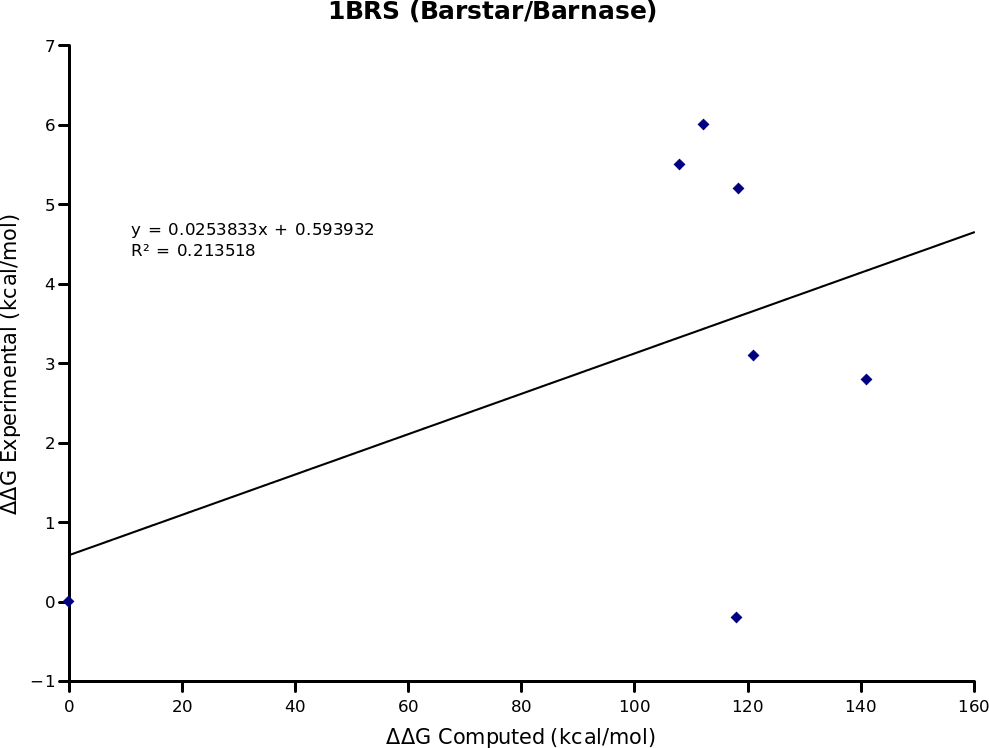
\includegraphics[width=0.65\textwidth]{figures/1brs_barstar_barnase.png}
    \caption{Computed versus experimental \ddg\ binding for 6 alanine mutations in the Barstar-Barnase binding pair.
    Crystal structure used for computations was 1BRS \protect\cite{buckle1994protein}.
    Specific amino acids mutated were residues 29, 35, 39, 42, 74, and 78, all of chain D.
    Experimental binding affinity taken from \protect\cite{thorn2001asedb}.}
    \label{figure:computational_mutation_scanning/1BRSd_ddg}
\end{figure}

\begin{table}[h]
\centering
\label{table:1brs_d_results}
\begin{tabular}{|c|c|c|}
\hline
Residue & \ddg\ calculated & \ddg\ experimental \\
\hline
native & 0 & 0 \\
29 & 121.07 & 3.1 \\
35 & 118.37 & 5.2 \\
39 & 118.09 & -0.2 \\
42 & 141.09 & 2.8 \\
74 & 107.92 & 5.5 \\
78 & 112.14 & 6 \\
\hline
\end{tabular}
\caption{Calculated and experimental \ddg\ for mutating given residues of barstar (chain D of structure 1BRS) to alanine.
Experimental values taken from \protect\cite{thorn2001asedb}.}
\end{table}

\begin{table}[!h]
\centering
\begin{tabular}{|c|c|c|}
\hline
Residue & Amino Acid & RMSD \\
\hline
D:29 & TYR & 0.121 \\
D:35 & ASP & 0.098 \\
D:39 & ASP & 0.335 \\
D:42 & THR & 0.114 \\
D:76 & GLU & 0.397 \\
D:80 & GLU & 1.804 \\
\hline
\end{tabular}
\caption{RMSD of mutated side chains in barstar, in a barnase-barstar complex (chain D of PDBid 1BRS), during the mutation scanning experiments.}
\label{table:1BRSd_rmsd}
\end{table}


\begin{figure}[h]
    \centering
    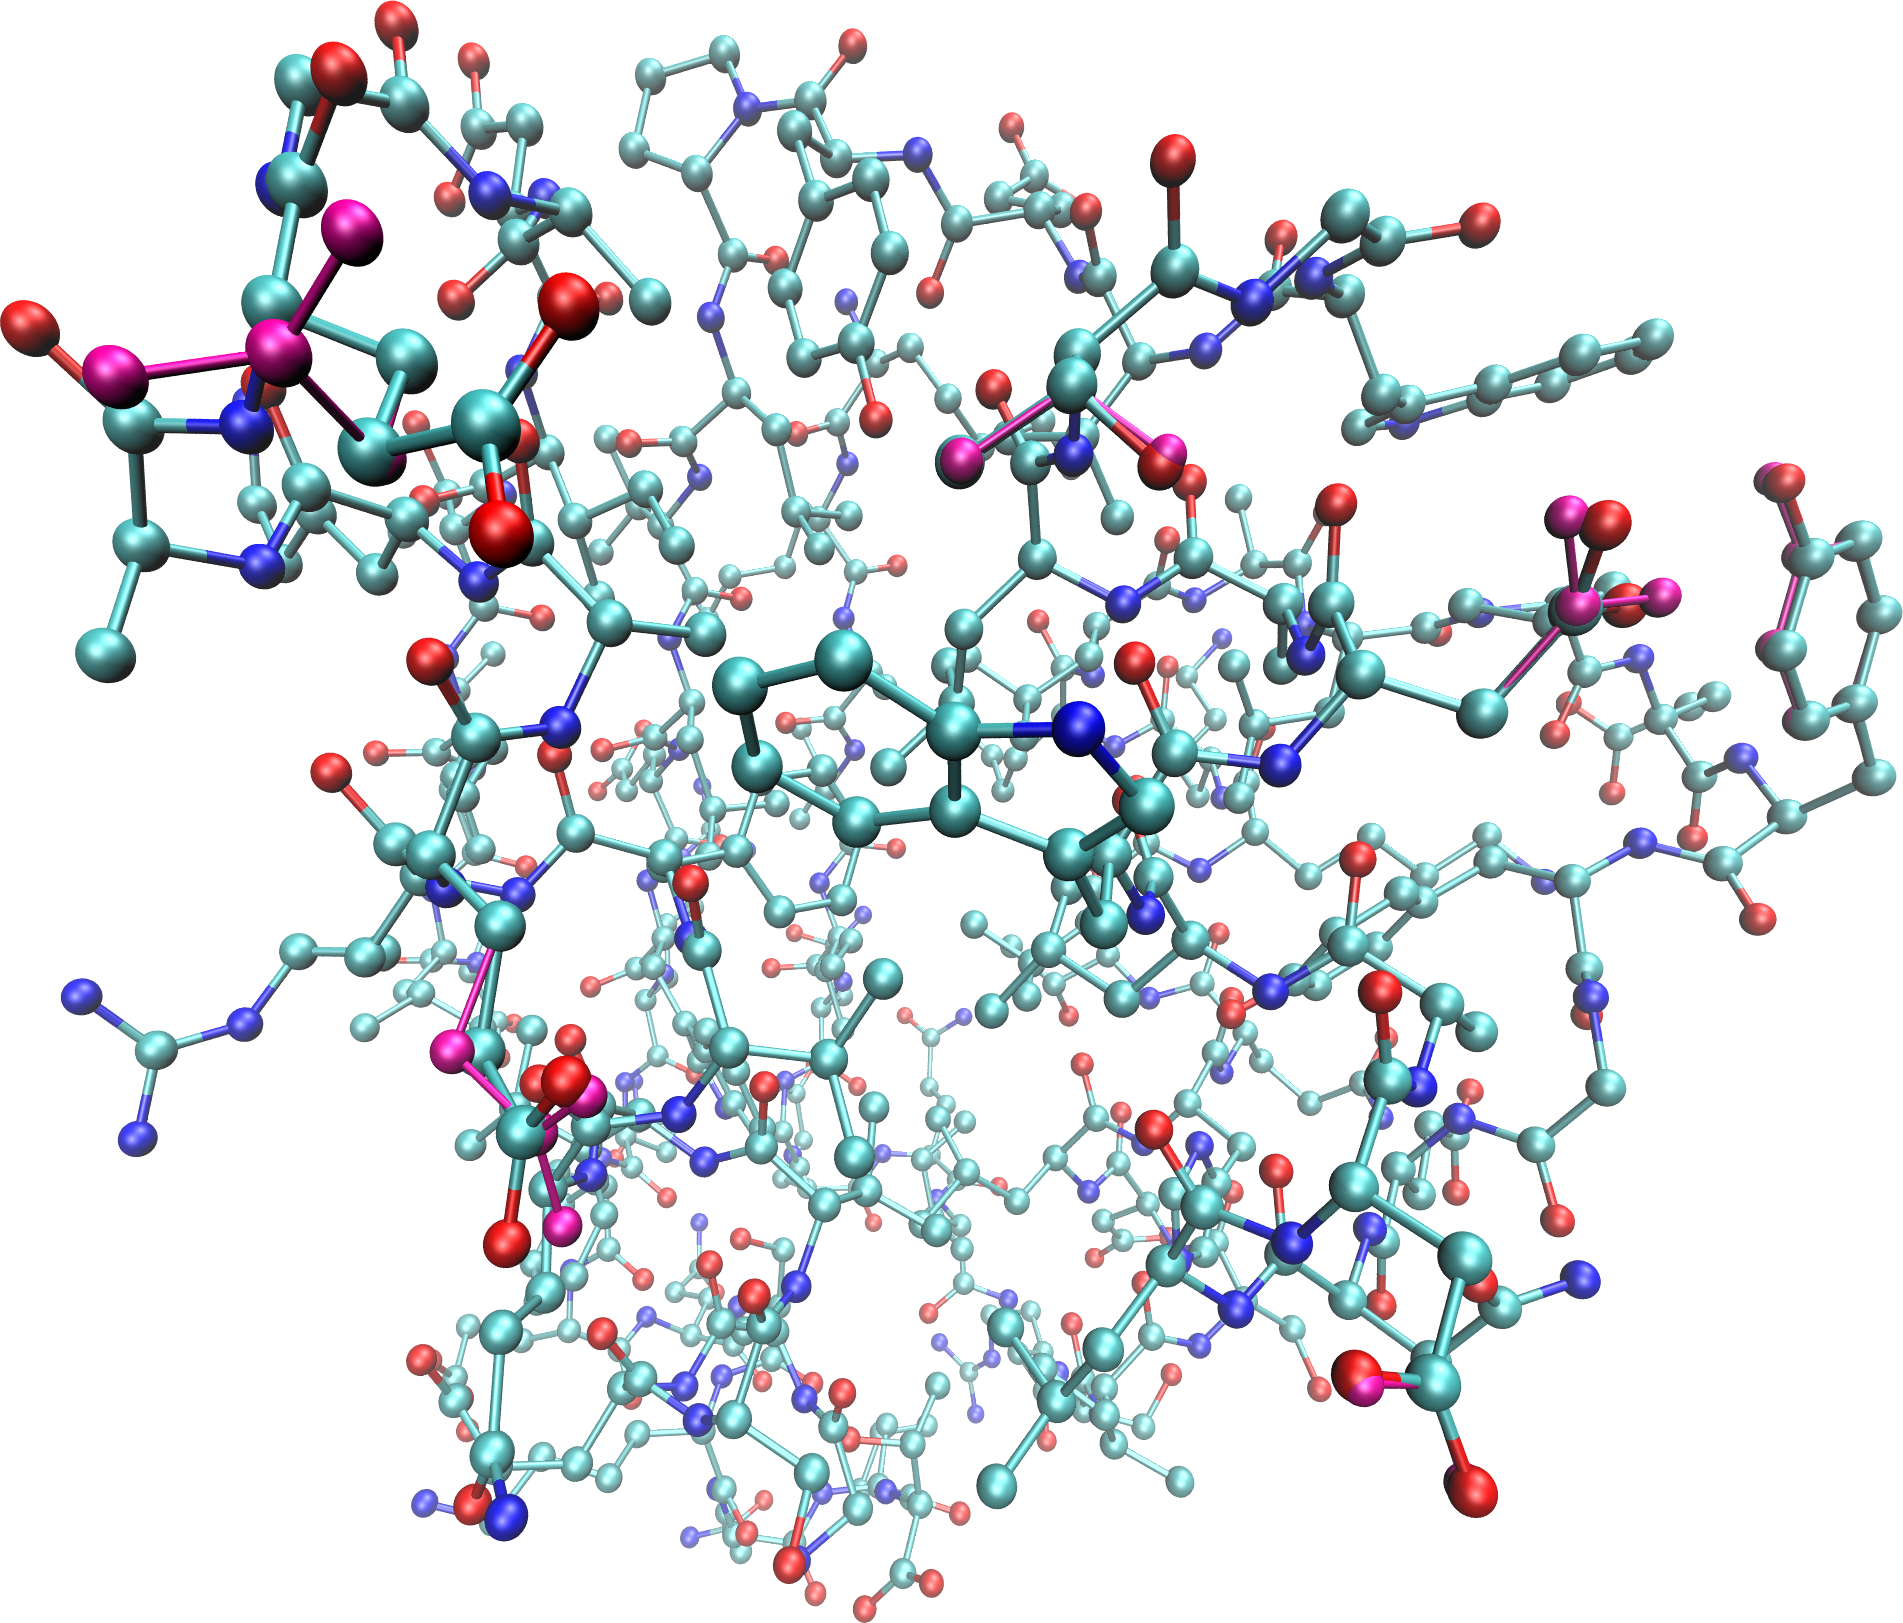
\includegraphics[width=0.65\textwidth,height=0.3\textheight,keepaspectratio]{figures/mutation_side_chain_images/1brs_all.png}
    \caption{Distribution of 6 mutated residues, shown in magenta, on the interface surface of barstar, 1BRS chain D.
    Five of the six residues are less than 0.4 angstroms RMSD to the crystal structure.
    The only exception is, glutamic acid 80, shown in the upper left of this figure, and also \protect\cite{figure:computational_mutation_scanning/1brs_d_80}.}
    \label{figure:computational_mutation_scanning/figname}
\end{figure}

\begin{figure}[h]
    \centering
    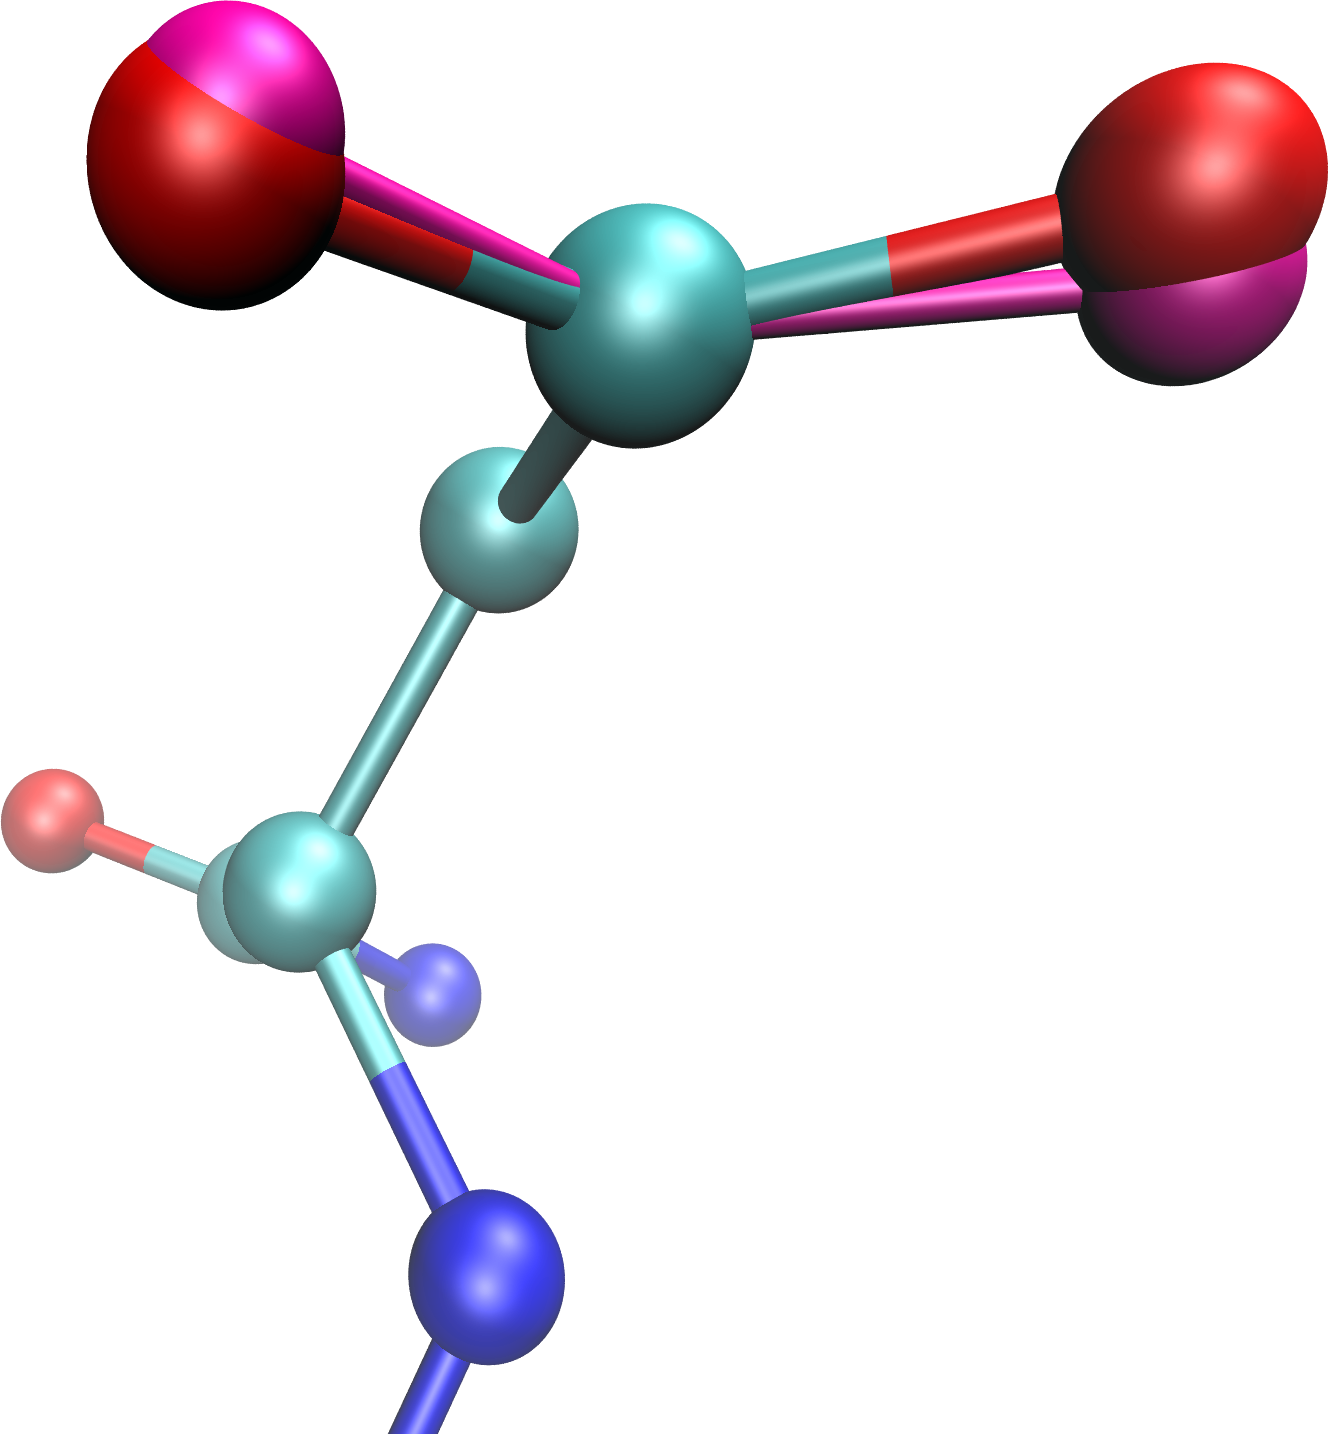
\includegraphics[width=0.65\textwidth,height=0.3\textheight,keepaspectratio]{figures/mutation_side_chain_images/1brs_chain_d_35.png}
    \caption{Crystal, colored by atom, and predicted, magenta, side chain conformations for barstar, chain D of PDBid 1BRS.
    The distance to the crystal structure is only 0.098 angstroms, or nearly identical.}
    \label{figure:computational_mutation_scanning/figname}
\end{figure}

\begin{figure}[h]
    \centering
    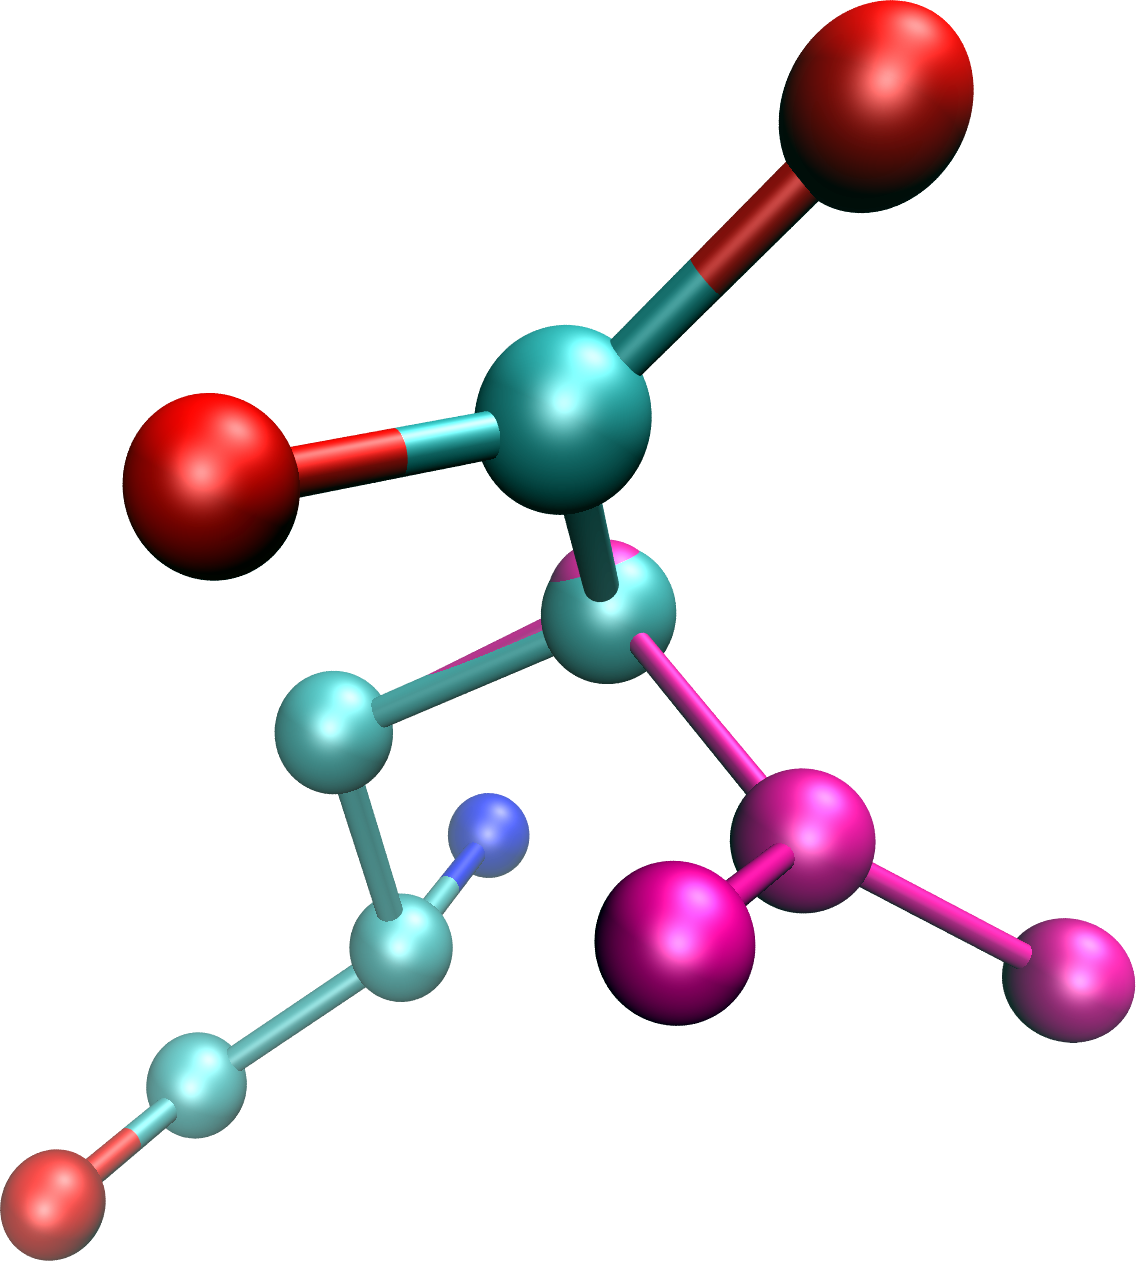
\includegraphics[width=0.65\textwidth,height=0.3\textheight,keepaspectratio]{figures/mutation_side_chain_images/1brs_chain_d_80.png}
    \caption{Glutamic acid 80 is the only residue on chain D, barstar, of the barnase-barstar complex which was not predicted within 0.4 angstroms of the crystal coordinates during the mutation scanning experiments.
    The difference between these two conformations is 1.804 angstroms, which while sometimes considered a ``successful'' prediction, is not sufficiently close to generate the same interactions, making it difficult to accurately predict binding affinities.}
    \label{figure:computational_mutation_scanning/1brs_d_80}
\end{figure}

% 1DVF
\clearpage
\begin{table}[H]
\centering
\label{table:energy_timings}
\begin{tabular}{|c|c|c|}
\hline
Residue & \ddg\ calculated & \ddg\ experimental \\
\hline
native & 0 & 0 \\
30 & -42.93 & 0.9 \\
32 & -44.68 & 1.8 \\
52 & -42.6 & 4.2 \\
54 & -28.29 & 4.3 \\
56 & -37.5 & 1.2 \\
58 & -41.91 & 1.6 \\
98 & -34.38 & 4.2 \\
99 & -30.51 & 1.9 \\
100 & -60.9 & 2.8 \\
101 & -37.84 & 4 \\
\hline
\end{tabular}
\caption{}
\end{table}

\begin{table}[!h]
\centering
\begin{tabular}{|c|c|c|}
\hline
Residue & Amino Acid & RMSD \\
\hline
B:30 & THR & 0.056 \\
B:32 & TYR & 0.412 \\
B:52 & TRP & 0.391 \\
B:54 & ASP & 0.442 \\
B:56 & ASN & 0.238 \\
B:58 & ASP & 0.159 \\
B:98 & GLU & 0.182 \\
B:99 & ARG & 1.137 \\
B:100 & ASP & 2.577 \\
B:101 & TYR & 0.340 \\
\hline
\end{tabular}
\caption{RMSD of mutated side chains in 1DVF, anti-hen-egg-white lysozyme antibody (D1.3) complexed with an anti-idiotopic antibody (E5.2), during the mutation scanning experiments.}
\label{table:1DVF_rmsd}
\end{table}


\begin{figure}[h]
    \centering
    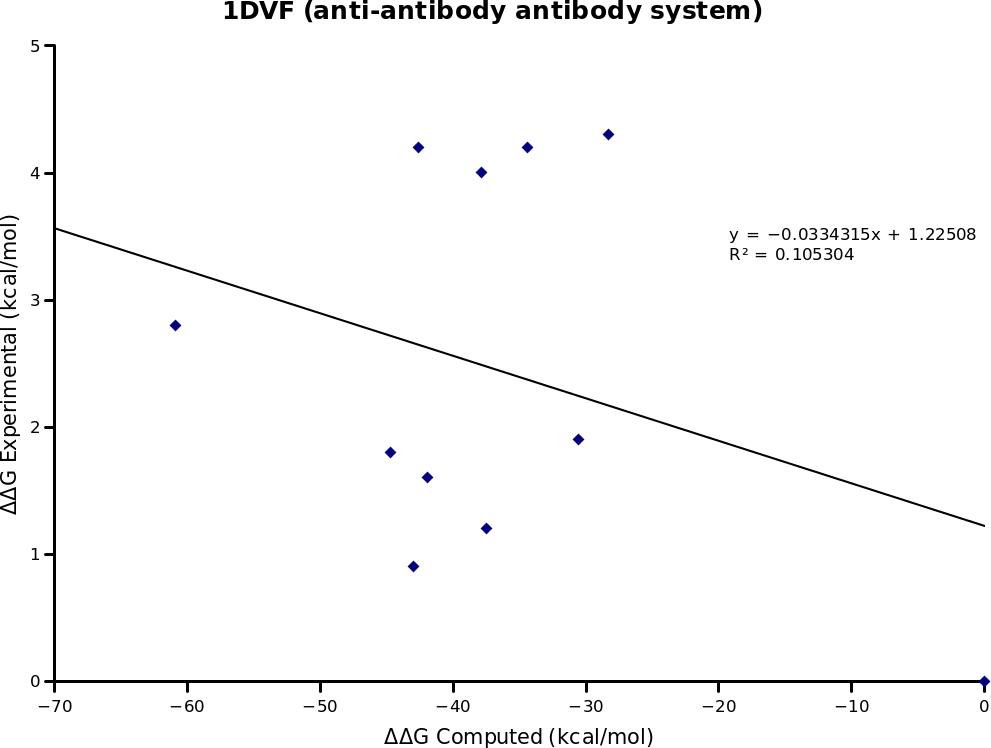
\includegraphics[width=0.65\textwidth]{figures/1dvf.png}
    \caption{Computed versus experimental \ddg\ binding for 10 alanine mutations in the anti-hen-egg-white lysozyme antibody (D1.3) anti-idiotopic antibody (E5.2) complex.
    Crystal structure used for computations was 1DVF \protect\cite{braden1996crystal}.
    Specific amino acids mutated were residues 30, 32, 52, 54, 56, 58, 98, 99, 100, and 101, all of chain A.
    Experimental binding affinity taken from \protect\cite{thorn2001asedb}.}
    \label{figure:computational_mutation_scanning/1DVF_ddg}
\end{figure}

\begin{figure}[h]
    \centering
    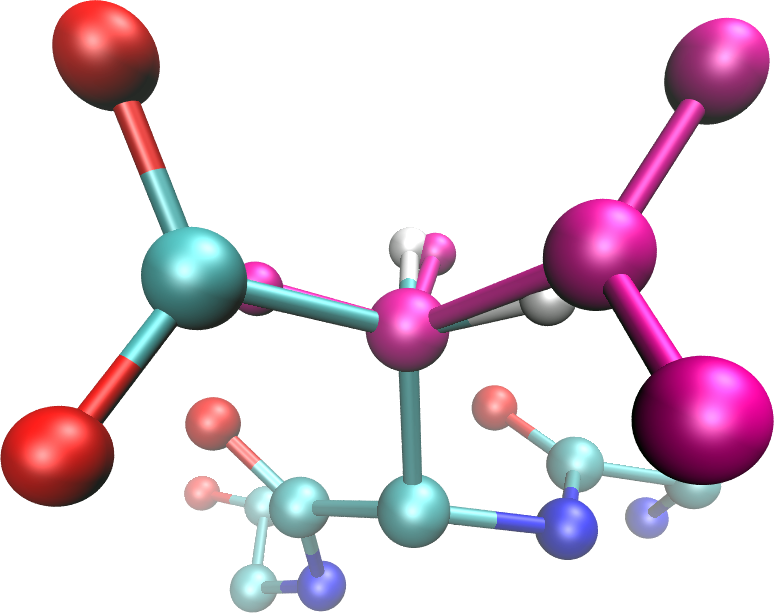
\includegraphics[width=0.65\textwidth,height=0.3\textheight,keepaspectratio]{figures/mutation_side_chain_images/1dvf_chain_b_100.png}
    \caption{An unsuccessful sidechain prediction in the antibody antigen complex of PDBid 1DVF.  
    The predicted conformation of this aspartic acid, B:100, differs from the native state by 2.577 angstroms.}
    \label{figure:computational_mutation_scanning/1DVF_b_100}
\end{figure}

\begin{figure}[h]
    \centering
    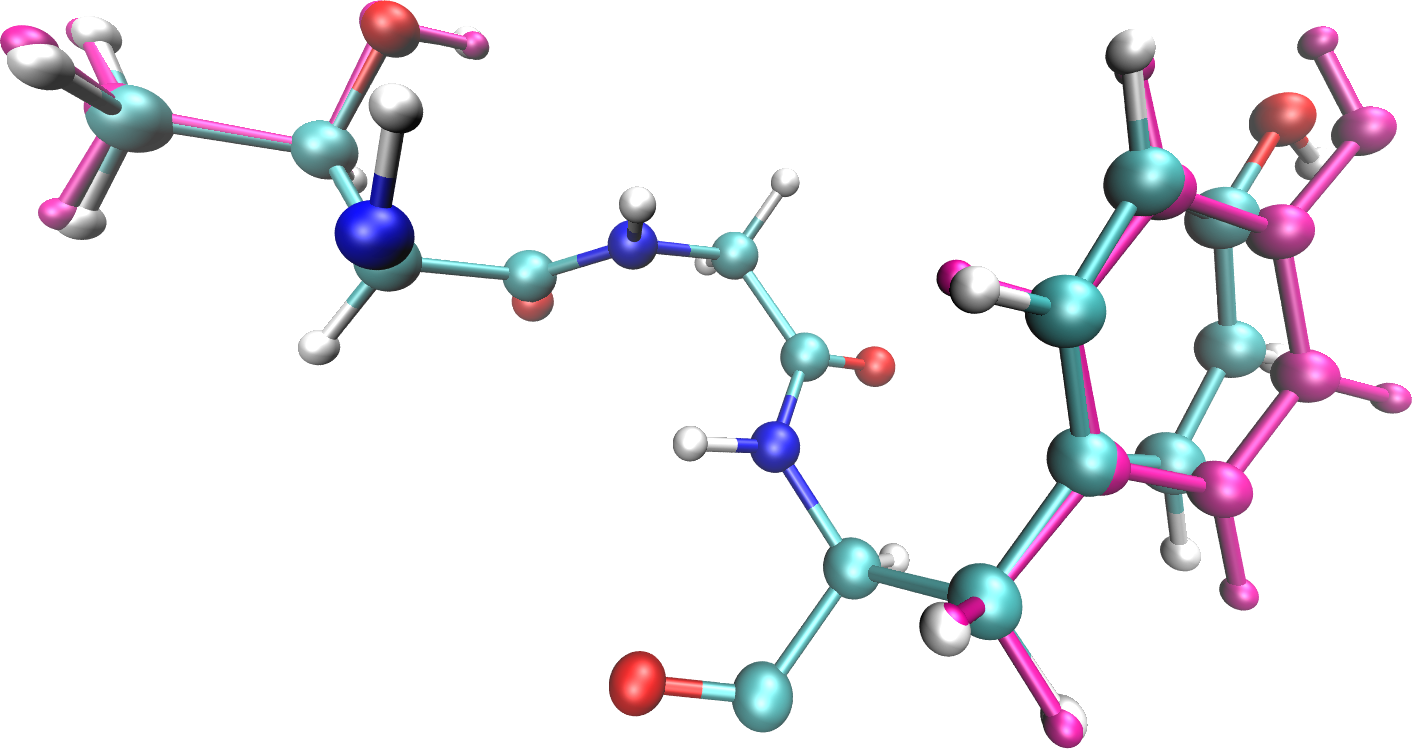
\includegraphics[width=0.65\textwidth,height=0.3\textheight,keepaspectratio]{figures/mutation_side_chain_images/1dvf_chain_b_30_and_32.png}
    \caption{Two neighboring successful predictions, shown in magenta, in the same antibody antigen complex.
    Threonine 30, left, is predicted almost identically to the native structure, at 0.056 angstroms from the crystal coordinates.
    Tyrosine 32, right, is predicted at 0.412 angstroms RMSD.
    Predicted structures are shown in magenta in both cases.}
    \label{figure:computational_mutation_scanning/1DVF_B_30_and_32}
\end{figure}

% 1FCC
\begin{table}[h]
\centering
\begin{tabular}{|c|c|c|}
\hline
Residue & \ddg\ calculated & \ddg\ experimental \\
\hline
native & -0.18 & 0 \\
25 & -4.55 & 0.24 \\
27 & 19.8 & 4.9 \\
28 & 26.37 & 1.3 \\
31 & 18.82 & 3.5 \\
35 & -6.31 & 2.4 \\
40 & -8.51 & 0.3 \\
42 & -5.56 & 0.4 \\
43 & 12.0 & 3.8 \\
\hline
\end{tabular}
\caption{Calculated and experimental \ddg\ for mutating given residues of Fc domain of human IgG (chain A of structure 1FCC) to alanine.
Experimental values taken from \protect\cite{thorn2001asedb}.}
\label{table:1FCC_results}
\end{table}

\begin{table}[!h]
\centering
\begin{tabular}{|c|c|c|}
\hline
Residue & Amino Acid & RMSD \\
\hline
C:25 & THR & 0.170 \\
C:27 & GLU & 0.403 \\
C:28 & LYS & 0.543 \\
C:31 & LYS & 0.594 \\
C:35 & ASN & 0.527 \\
C:40 & ASP & 1.292 \\
C:42 & GLU & 2.994 \\
C:43 & TRP & 0.371 \\
\hline
\end{tabular}
\caption{RMSD of mutated side chains in 1FCC, C2 fragment of streptococcal protein G in complex with the Fc domain of human IgG, during the mutation scanning experiments.}
\label{table:1FCC_rmsd}
\end{table}


\begin{figure}[h]
    \centering
    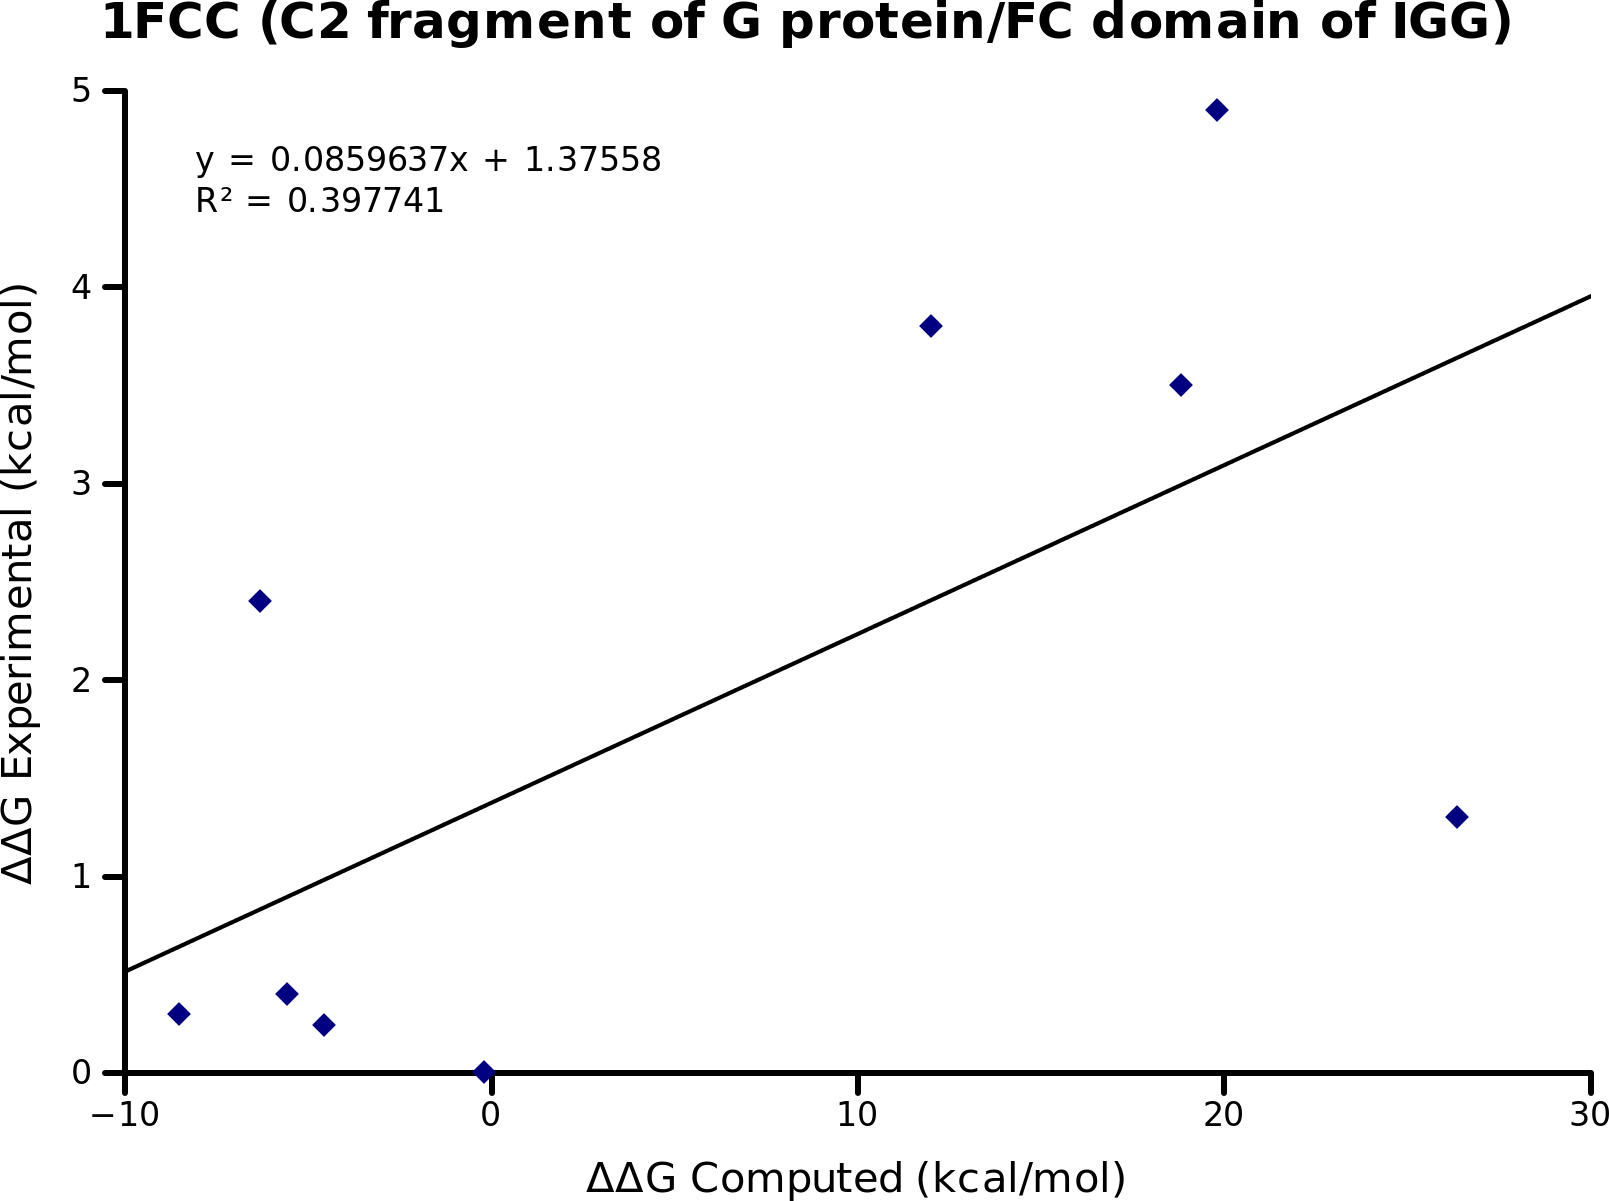
\includegraphics[width=0.65\textwidth]{figures/1fcc.png}
    \caption{Computed versus experimental \ddg\ binding for 8 alanine mutations in  binding pair.
    Crystal structure used for computations was 1FCC.
    Specific amino acids mutated were residues 25, 27, 28, 31, 35, 40, 42, and 43, all of chain A.
    Experimental binding affinity taken from \protect\cite{thorn2001asedb}.}
    \label{figure:computational_mutation_scanning/1FCC_ddg}
\end{figure}

\begin{figure}[h]
  \centering
  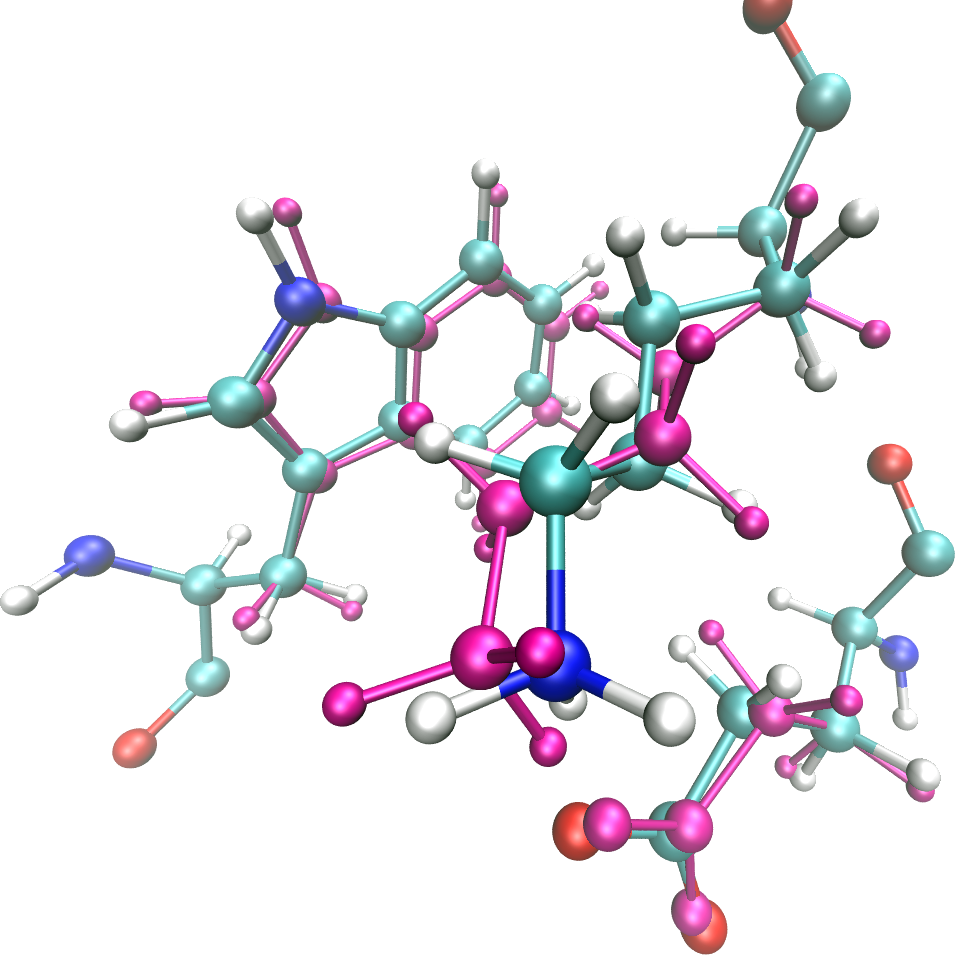
\includegraphics[width=0.65\textwidth,height=0.3\textheight,keepaspectratio]{figures/mutation_side_chain_images/1fcc_27_31_43.png}
  \caption{Three clustered hot spot residues in another antibody antigen complex, PDBid 1FCC, the C2 fragment of streptococcal protein G in complex with the Fc domain of human IgG.
The predicted conformations for glutamic acid 27, lysine 31 and tryptophan 43 are depicted in magenta.
All three of these side chains are in good agreement with the crystal structure, with side chain RMSD's of 0.403, 0.594 and 0.371 respectively.
These residues are shown in greater detail in other figures, glutamic acid 27 in figure \protect\ref{figure:computational_mutation_scanning/1FCC_27}, lysine 31 in figure \protect\ref{figure:computational_mutation_scanning/1FCC_31}, and tryptophan 43 in figure \protect\ref{figure:computational_mutation_scanning/1FCC_43}.
Tryptophan 43 is interesting in that despite being critical to protein-protein binding it is largely buried in a pocket defined by the neighboring protein structure.
This interaction is examined in figure \protect\ref{figure:1fcc_43_pocket}.}
  \label{figure:computational_mutation_scanning/1FCC_27_31_43}
\end{figure}

\begin{figure}[h]
  \centering
  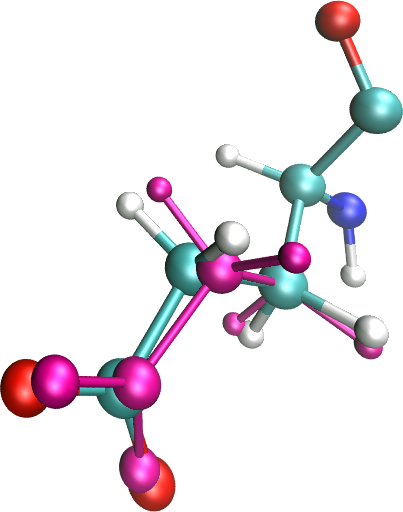
\includegraphics[width=0.65\textwidth,height=0.3\textheight,keepaspectratio]{figures/mutation_side_chain_images/1fcc_27.png}
  \caption{Predicted, magenta, and crystal conformations, colored by element, for glutamic acid 27.
The side chain RMSD of this prediction is 0.403 angstroms.
This side chain is in close proximity to a number of other hot spot residues on the protein protein interface and is shown in context in figure \protect\ref{figure:computational_mutation_scanning/1FCC_27_31_43}.}
  \label{figure:computational_mutation_scanning/1FCC_27}
\end{figure}

\begin{figure}[h]
  \centering
  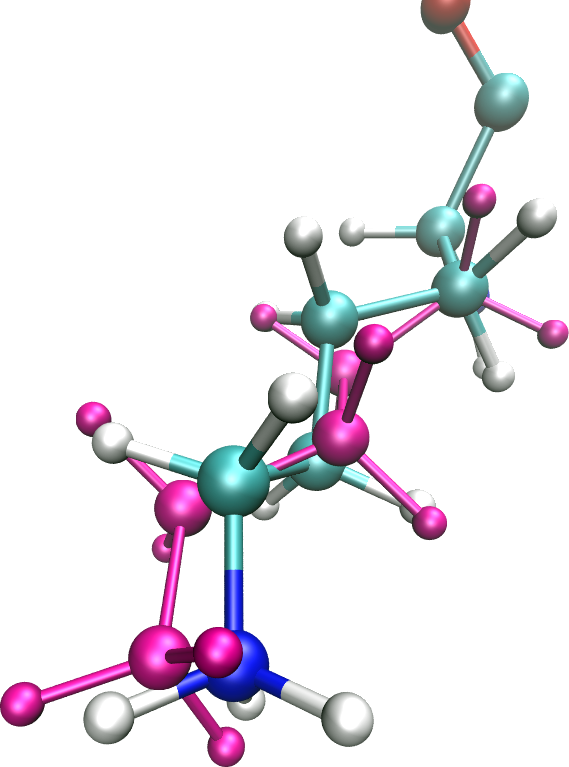
\includegraphics[width=0.65\textwidth,height=0.3\textheight,keepaspectratio]{figures/mutation_side_chain_images/1fcc_31.png}
  \caption{The predicted side chain conformation during the course of mutation scanning experiments, shown in magenta, compared to the native conformation, shown colored by atom for lysine 31.
The RMSD of this prediction is 0.594 angstroms.}
  \label{figure:computational_mutation_scanning/1FCC_31}
\end{figure}

\begin{figure}[h]
  \centering
  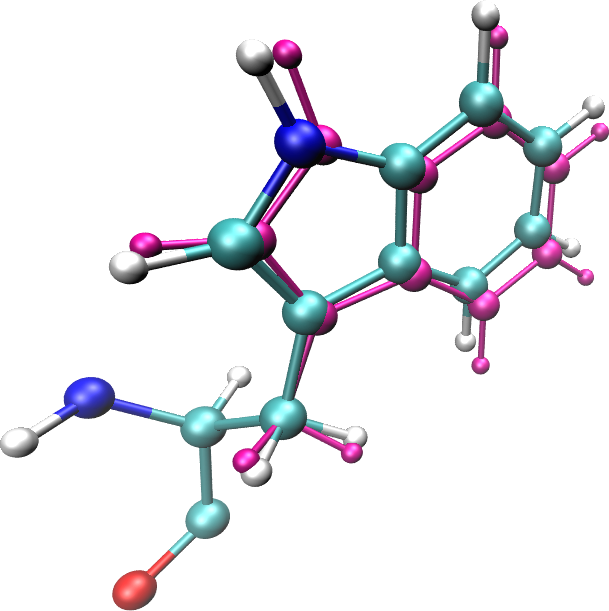
\includegraphics[width=0.65\textwidth,height=0.3\textheight,keepaspectratio]{figures/mutation_side_chain_images/1fcc_43.png}
  \caption{Native, colored by element, and predicted, magenta side chain conformation for tryptophan 43 of 1FCC.
The root mean square distance of the predicted conformation to the native is 0.371 angstroms.
The effect of the local protein structure on the conformation of this residue is examined in figure \protect\ref{figure:1fcc_43_pocket}.}
  \label{figure:computational_mutation_scanning/1FCC_43}
\end{figure}

\begin{figure}
    \centering
    \begin{subfigure}[b]{0.3\textwidth}
        \centering
        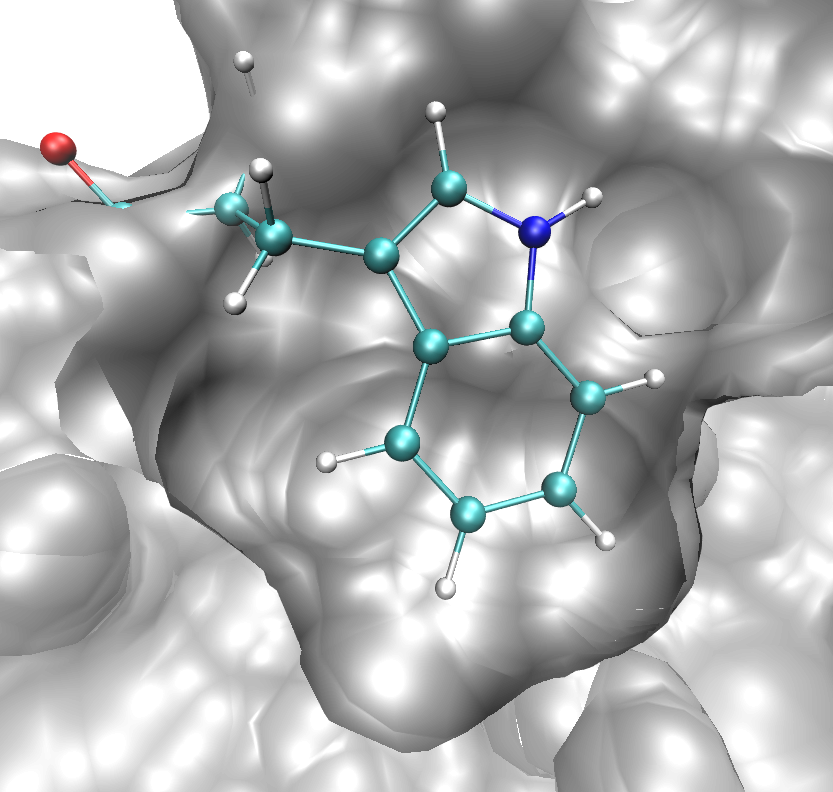
\includegraphics[width=\textwidth,height=\textheight,keepaspectratio]{figures/mutation_side_chain_images/in_pocket_out_of_plane.png}
        \caption{}
        \label{figure:mutation_side_chain_images/in_pocket_out_of_plane}
    \end{subfigure}
    \hspace{0.1\textwidth}
    \begin{subfigure}[b]{0.3\textwidth}
        \centering
        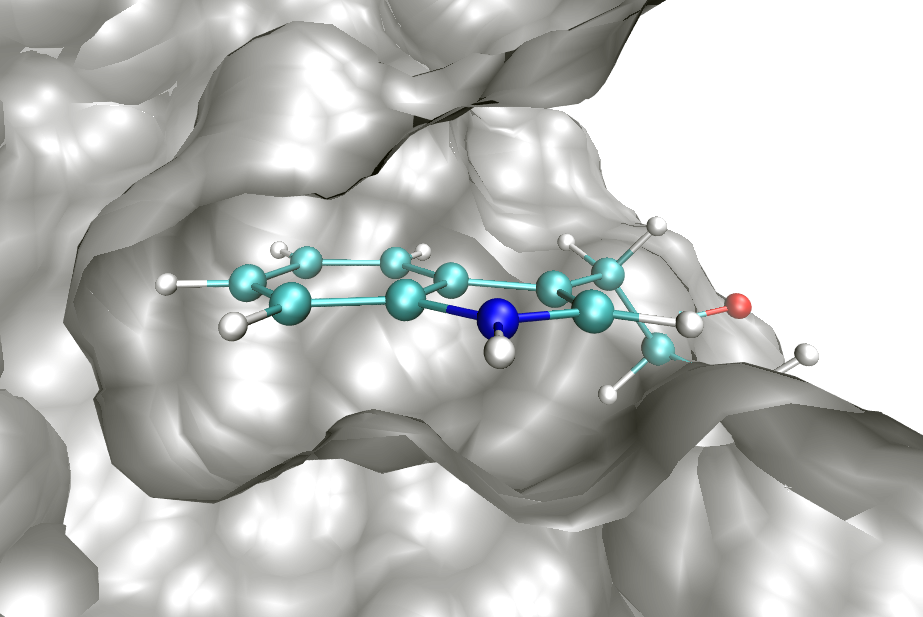
\includegraphics[width=\textwidth,height=\textheight,keepaspectratio]{figures/mutation_side_chain_images/in_pocket_in_plane.png}
        \caption{}
        \label{figure:mutation_side_chain_images/in_pocket_in_plane.png}
    \end{subfigure}
    \caption{The pocket of tryptophan 43 of 1FCC.  
Because of conformation of the neighboring protein structure this residue has very little conformational freedom, and any prediction which successfully locates the sidechain in the pocket will be reasonably close to the native state.
The conformation predicted in these experiments was very similar, 0.371 angstroms, and is depicted superimposed with the native in figure \protect\ref{figure:computational_mutation_scanning/1FCC_43}.}
    \label{figure:1fcc_43_pocket}
\end{figure}


